\section{Implementation details}

Our implementation falls broadly under cognitive modeling, which seeks to simulate human cognitive processes and problem-solving through a computerized model. We advocate for exposure-based learning in music, encouraging active engagement with as many musical styles, genres, techniques, and learning methods as possible. This approach promotes comprehensive musical proficiency and efficient performance when encountering novel and unseen data in practical applications.

According to Piaget's theory of cognitive development, children gain knowledge through sensory experiences and gradually develop abstract reasoning and schemas—basic cognitive structures \cite{Huitt2003PiagetsDevelopment}. These schemas evolve by incorporating new information through assimilation and accommodation \cite{audioselfsupsurvey}.

In pattern recognition, models are designed to exhibit robustness against known invariances—transformations of input data ---thereby ensuring consistent output. Even unknown invariances not explicitly considered in the model's design can be accommodated due to the model's inherent learning capacity.

Our implementation slightly modifies the Contrastive Learning of Music Representations (CLMR) method \cite{CLMR2021}, which learns valuable, discriminative music representations without explicit labels by contrasting positive augmentations of a musical piece against negative ones. CLMR falls under a branch of ML known as self-supervised learning (SSL) \cite{Balestriero2023ALearning}, where models learn autonomously from unlabeled data to create their own supervisory signals \cite{audioselfsupsurvey}. This method resembles how humans learn from observations and interactions, transforming unsupervised problems into supervised ones by auto-generating labels. SSL benefits include reduced dependence on labeled data, contributing to more robust and generalizable data representations.

Although SSL has proven effective in speech and audio, its application to music audio remains relatively unexplored. This is primarily due to the unique challenges of modeling musical knowledge, especially regarding music's tonal and pitched characteristics \cite{Li2023MERT:Training}.

\subsection{Deep architecture design}

This work suggests employing a Triplet Siamese Network (TSN), a model architecture known for its efficacy in music similarity retrieval tasks \cite{contentmusicsimtriplet2020}. The aim is to minimize the loss function between a triplet of anchor, positive, and negative samples, utilizing online triplet mining for optimizing memory resources \cite{Sikaroudi2020OfflinePatches}. This SSL model aims to distinguish between similar and dissimilar samples effectively.

Introduced by Bromley and LeCun \cite{Bromley1993SignatureNetwork}, Siamese Networks are DL architectures designed for tasks requiring comparison or similarity assessment between instances. The architecture comprises identical subnetworks that share the same parameters, improving memory usage and computational efficiency. Rather than learning specific features of individual classes, they focus on a similarity metric, making them ideal for imbalanced datasets. Each subnetwork processes an input independently, combining the outputs to yield a similarity score. Training with shared weights enables the model to learn invariant input representation, improving comparison efficiency. This is accomplished through a specialized loss function called triplet loss, which aims to minimize the distance between similar inputs and maximize it for dissimilar ones. The loss function will be explained later in Subsection~\ref{subsec:loss-function}.

The TSN extends the traditional binary contrastive architecture by comparing three input instances instead of two. It strives to learn an embedding space where similar instances are closer and dissimilar ones are more distant.

\subsubsection{Encoder: SampleCNN}

The SampleCNN model \cite{Lee2018SampleCNN:Classification} is a CNN designed for raw waveform audio data, treating each audio sample as an independent channel and applying 1-dimensional convolution along the temporal axis. Our implementation is an adaptation of \cite{CLMR2021} using \textit{PyTorch} \cite{Paszke2019PyTorch:Library} and \textit{PyTorch Lightning} \cite{PyTorchDocumentation}.

With only 2.4 million trainable parameters, this fully convolutional model reduces computational requirements and learns features at different scales through its multi-resolution architecture. See layer specifications in Table \ref{tab:samplecnntable}.

%%%%%%%%%%%%%%%%%%%%%%%%%%%%%

\begin{figure}
    \centering
    \includegraphics{figures/images/applsci-08-00150-g003.png}
    \caption[SampleCNN filters]{\small{The spectrum of the estimated filters in the intermediate layers of SampleCNN is sorted by the frequency of the peak magnitude. The x-axis represents the index of the filter, and the y-axis represents the frequency range from 0 to 11 kHz. The model used for visualization is  39---SampleCNN with 59,049 samples as input. \cite{Lee2018SampleCNN:Classification}}}
    \label{fig:filters}
\end{figure}

%%%%%%%%%%%%%%%%%%%%%%%%%%%%%

\begin{table}[ht]
\centering
\small
\begin{tabularx}{\textwidth}{
  >{\centering\arraybackslash\hsize=0.4\hsize}X
  >{\centering\arraybackslash\hsize=0.2\hsize}X
  >{\centering\arraybackslash\hsize=0.2\hsize}X
  >{\centering\arraybackslash\hsize=0.2\hsize}X}
\toprule
\thead{\textbf{Layer Type}} & \thead{\textbf{In Channels}} & \thead{\textbf{Out Channels}} & \thead{\textbf{Num. of layers}} \\
\midrule
Conv + ReLU & 1 & 128 & 1 \\
Conv + BatchNorm + ReLU + MaxPool & 128 & 128 & 2 \\
 & 128 & 256 & 1 \\
 & 256 & 256 & 6 \\
 & 256 & 512 & 1 \\
Conv + BatchNorm + ReLU + AvgPool & 512 & 512 & 1 \\
Fully connected layer & 512 & 128 & 1 \\
\bottomrule
\end{tabularx}
\caption[SampleCNN layer specifications]{\small{Layer specifications for our SampleCNN model implementation; extracted and extended from \cite{CLMR2021}.}}
\label{tab:samplecnntable}
\end{table}


The original model has been subtly adjusted by introducing an average pooling operation to the final convolutional layer. This modification is strategic for handling various input data sizes. Condensing the feature maps to a fixed-size output ensures consistency for subsequent layers like fully connected ones, streamlining computations while maintaining crucial information.

\subsection{Optimizer and learning rate}

We've employed the AdamW optimizer \cite{Loshchilov2017DecoupledRegularization}, an optimized variant of the widely-used Adam optimizer for training neural networks. AdamW adeptly balances the learning rate across network weights, providing an efficient strategy for weight decay management by isolating it from gradient updates. 

The learning rate, set at 0.003, is a pivotal parameter dictating the step size at each iteration towards loss function minimization. It's a delicate balancing act ---a high rate promises swift convergence with a risk of minimum overshoot, while a lower rate provides careful convergence but necessitates more iterations. Given that delicacy, we set it to a standard number broadly used in the literature.

\subsection{Audio augmentation and transformation pipeline}

The choice of input data is guided by the task, computational resources, and the need to balance data retention with computational efficiency.

Previous research has utilized CNNs with various features such as Mel-Scaled Log-magnitude Spectograms (MLS), Self-Similarity Matrices (SSM), and Self-Similarity Lag Matrices (SSLM) as inputs \cite{Hernandez-Olivan2021MusicFeatures}. However, features derived from raw audio may lack interpretability in some scenarios \cite{Schindler2020DeepTutorial}, and raw audio presents unique advantages despite being highly computationally demanding. It ensures the preservation of the original signal, potentially uncovering novel insights, and allows for direct feature extraction via advanced DL models \cite{learning, verydeep}. Nevertheless, it comes with challenges, such as high ---the highest--- dimensionality requiring substantial computational resources. 

Time-domain processing naturally handles temporal patterns and sequences in data, thereby avoiding windowing artifacts. Although audio feature-based methods are effective for various audio-related machine learning tasks, their limitations lie in representing perceptual similarity. MLS, for example, captures frequency distribution over time. Yet, the complexity of human auditory perception, encompassing temporal patterns, phase relationships between frequencies, and higher-level musical structures means that musically similar sounds can have distinct spectrograms. This discrepancy implies that using spectrogram distance alone for measuring high-level music content may not always align with human perceptions \cite{Kim2020OneStrategies, Mesostructures2023}.

In conclusion, raw audio waveforms were our final choice for input for the anchor. Each input sequence was 15 seconds long, roughly equivalent to 8 bars of 4/4 music at 120 beats per minute. The audio was sampled at a frequency of 16 kHz, a decision influenced by computational resources. We are confident that this choice of input contains a significant amount of meaningful musical information. Although it may not encompass the complexity of a symphony, it is sufficient for the scope of our experiments.

\subsubsection{Positive sample generation chain}

The positive waveform in every triplet of input data must preserve its intelligible content when subjected to transformations, regardless of alterations in sonic qualities and processing artifacts. Maintaining the temporal structure and meaningfulness of the content allows it to present musical elements remarkably close to the original track.

While we have experimented with helpful audio augmentation tools such as \cite{Spijkervet2021Spijkervet/torchaudio-augmentations:V1.0, Kharitonov2020DataDomain}, the specific requirements of our experiments required the development of our own transformation chain using \textit{torchaudio}'s \cite{Yang2021TorchAudio:Processing} implementation of \textit{SoX} \cite{sox}: given an anchor audio signal $A[n]$, we generate a positive signal $P[n]$ by applying a series of amplitude, time-domain, frequency-domain, modulation, reverberation, and nonlinear effects with additive noise on top of it. 

\textbf{Amplitude effects}: The signal's amplitude is modified by a constant factor using gain $g \in [-12, 0]$. 

\textbf{Time-domain effects}: The signal's playback speed and duration are altered through speed change and stretching, preserving the relative perceptual musical relationships between wave points. The respective factors are $\alpha \in [0.9, 1.1]$ for speed change and $\beta \in [0.9, 1.1]$ for stretch. 

\textbf{Frequency-domain effects}: The frequency content is adjusted through pitch-shifting, modifying the pitch by $\Delta p \in [-1200, 1200]$ cents. 

\textbf{Nonlinear effects}: Nonlinear distortion is introduced via overdrive with a parameter $d \in [0, 30]$. 

\textbf{Modulation effects}: Utilize a control signal or low-frequency oscillator. Six variables determine the \href{https://github.com/oriolcolomefont/Uncovering-High-Level-Content-in-the-Time-Domain/blob/24057f4160a4ecb7ccef16146ad086ab5160aef8/dataset.py#L120C9-L128C10}{chorus parameters}. The tremolo's amplitude modulation frequency and depth are controlled by $t_s \in [0.1, 100]$ and $t_d \in [1, 101]$, respectively. 

\textbf{Reverberation effects} simulate a physical space's acoustic reflections and reverberations by applying an impulse response.

\textbf{Noise effects}: A noise signal $Noise[n]$ is added with a signal-to-noise ratio (SNR) in the range $[12, 100]$. 

The positive signal $P[n]$ is generated by convoluting the various impulse responses of specific effects. The noise signals are included with a set SNR ratio within the above range on top of the effect chain.

Random parameter updates within hardcoded ranges generate unique audio $P[n]$ images out of $A[n]$ anchor for each run-through. Adding random white noise and varying SNR creates countless noisy waveform variations. Although possible combinations can be estimated by multiplying discrete parameter values, the presence of continuous parameters and randomness in noise generation effectively results in infinite unique audio versions.

\subsubsection{Negative sample generation}

Circling back to our premises and assumptions, we posit that high-level musical content unfolds over time; therefore, we argue that the temporal structure of the negative images, in contrast to our anchor, must be disrupted. While maintaining similar sonic qualities, the content should be rendered unintelligible.

The computation for the negative signal $N[n]$ per every $A[n]$ goes as follows:

\begin{enumerate}
\item We first calculate the minimum and maximum audio chunk lengths in samples:
\begin{align}
l_{min} &= t_{min} \times S, &
l_{max} &= t_{max} \times S
\end{align}

The minimum duration $t_{min}$ is set to 0.05 seconds, and the maximum duration $t_{max}$ is set to 1 second. This range is chosen thoughtfully to strike a balance between two factors: on the one hand, it is above the just noticeable difference (JND) threshold, the smallest change in a stimulus that can be perceived. On the other hand, it is short enough to maintain a reasonably-sized window to avoid discernible musical content \cite{Fastl2007Just-NoticeableChanges}.

\item We then generate random audio chunk lengths $l_1, l_2, \ldots, l_{n-1}$ from the uniform distribution on the interval $[l_{min}, l_{max}]$. Calculate the final audio chunk length as:
\begin{equation}
l_n = L_A - \sum_{i=1}^{n-1} l_i
\end{equation}
where $L_A$ is the length of the anchor signal in samples.

\item The third step is to split the anchor signal $A$ into audio chunks $C_1, C_2, \ldots, C_n$ according to the calculated audio chunk lengths in the previous step.

\item Shuffle the audio chunks randomly to get the permuted slices $C_{\sigma(1)}, C_{\sigma(2)}, \ldots, C_{\sigma(n)}$, where $\sigma$ is a random permutation of indices from $1$ to $n$. 

\item We finally concatenate the shuffled audio chunks to generate the negative signal that will have similar production while the content is completely ruined:
\begin{equation}\label{eq:negative_signal}
N[n] = C_{\sigma(1)} \oplus C_{\sigma(2)} \oplus \ldots \oplus C_{\sigma(n)}
\end{equation}
\end{enumerate}

The whole purpose of this process is to disturb the content unfolding in the time domain so it becomes musically unintelligible while maintaining the production and sonic attributes.

\subsection{Loss function}
\label{subsec:loss-function}

Schroff, F., Kalenichenko, D., and Philbin, J. from Google first proposed and applied triplet loss for the learning of facial recognition, catering to varied poses and angles of the same individual \cite{Schroff2015FaceNet:Clustering}.

Contrary to the widespread contrastive loss \cite{supercontrast}, the triplet loss function directs the learning process by minimizing the distance between the anchor and positive instances and maximizing the distance between the anchor and negative instances. Including a margin parameter in the loss function guarantees a minimum separation between positive and negative instances in the embedding space.

The triplet loss function $\mathcal{L}(\mathbf{a}, \mathbf{p}, \mathbf{n})$ aims to ensure that an anchor vector $\mathbf{a}_i$ is closer in the embedding space to a positive vector $\mathbf{p}_i$ (representing an example of the same class) than to a negative vector $\mathbf{n}_i$ (representing an example of a different class) by at least a margin $\alpha$. It is calculated by summing the losses overall $N$ triplets in the dataset, where the equation gives the loss for each triplet:

\begin{equation}
\mathcal{L}(\mathbf{a}, \mathbf{p}, \mathbf{n}) = \sum_{i=1}^{N} \max \left(0, \left| \mathbf{a}_i - \mathbf{p}_i \right|_2^2 - \left| \mathbf{a}_i - \mathbf{n}_i \right|_2^2 + \alpha \right)
\end{equation}

The $\max(0, x)$ operation ensures zero loss when the distances satisfy this condition. The final loss used for model training is then the average loss over a mini-batch of $N$ triplets:

\begin{equation}
\mathcal{L} = \frac{1}{N} \sum_{i=1}^{N} \mathcal{L}(\mathbf{a}_i, \mathbf{p}_i, \mathbf{n}_i)
\end{equation}

The margin is a task-dependent optimal value determined empirically based on model performance. If it's too small, the model might not differentiate classes effectively; if it's too large, it might focus on outliers.

While some packages can be found in the MIR online community \cite{auraloss}, we wrote our own \textit{PyTorch} \cite{Paszke2019PyTorch:Library} implementation for the sake of our experiments.

As previously stated, the goal of minimizing this loss function is to learn discriminative embeddings, where similar examples are grouped closely together. In contrast, dissimilar examples are placed farther apart in the embedding space.

\subsection{Online triplet mining and batch normalization}

Online triplet mining is beneficial for managing large datasets by dynamically selecting the most informative triplets during training, focusing on each mini-batch. This strategy makes the process memory-efficient by negating the need to store all possible triplet combinations. Still, it also enhances model performance through quicker convergence by focusing on challenging examples based on the current model state.

This hard triplet mining selects triplets $(a, p, n)$ to maximize the Euclidean distance between the anchor and positive samples and the anchor and negative samples. These distances, $D_{\text{AP}}$ and $D_{\text{AN}}$, are computed respectively:

\begin{align}
D_{\text{AP}} &= \sqrt{\sum_{i} (A_i - P_i)^2} & D_{\text{AN}} &= \sqrt{\sum_{i} (A_i - N_i)^2}
\end{align}

In implementing the batch normalization step, it is necessary to standardize the audio lengths across all elements in the minibatch. We opted to zero-pad all clips to the length of the longest clip, valuing data integrity and completeness over potential performance trade-offs. Thus, the length of the longest array in the batch, which sets the standard for all others, is as follows:

\begin{equation}
L_{\text{max}} = \max_{i \in I} \left( \max \left( |A_i|, |P_i|, |N_i| \right) \right)
\end{equation}

$I$ represents the set of all items in the batch, $|A_i|$, $|P_i|$, and $|N_i|$ denote the lengths of the anchor, positive, and negative vectors for the $i$-th item, respectively. The $\max$ function is applied to find the longest of these three lengths for each item, and then the maximum of these maximum lengths is taken over all items in the batch. This gives the maximum length, $L_{\text{max}}$, of any vector in the batch.

\subsubsection{Hardware and training strategy}

The deep learning models were trained on a high-performance cloud computing setup hosted on \href{https://cloud.google.com/}{the Google Cloud Platform}. The machine was of type \texttt{n1-standard-32}, equipped with an Intel Skylake processor and four NVIDIA Tesla T4 GPUs. The multiple GPUs allowed for efficient parallel processing, significantly reducing the training time.

To tackle the computational demands of training models on extensive raw audio data, we incorporated a couple of strategies to optimize efficiency and performance. 

First, we utilized 16-mixed precision training. This approach leverages the improved performance of modern GPUs for 16-bit computations, enabling the model to run faster and use less memory without sacrificing model performance \cite{Das2018MixedOperations}.

Secondly, to capitalize on the computational capabilities of multiple GPUs and hasten training times, we employed the Distributed Data-Parallel (DDP) strategy \cite{Li2020PyTorchTraining}. DDP operates on distinct mini-batches of data across GPUs and synchronizes the gradients after each backward pass, providing a more efficient scaling than other parallel strategies. 

These strategies collectively enhance the computational efficiency while maintaining the robustness of the model training on lengthy raw audio data.

\subsection{The \textit{embeddiogram}, a deep audio feature representation}

The \textit{embeddiogram}, a deep audio feature representation, is derived by applying our pre-trained neural network to sliding windowed segments across the audio signal, generating a sequence of embedding vectors. These relatively low-dimensional vectors collectively form a two-dimensional description of the audio signal's musical content. A visual representation can be seen in Figure \ref{fig:embeddiogram}.

Below is a detailed explanation of how we compute the \textit{embeddiogram} from a given audio signal of length $N$. This process comprises loading the audio data, slicing the audio data into windowed segments, processing each window using our pre-trained model to produce a vector per window/time frame, collecting and stacking these embeddings, and finally, normalizing the resulting matrix. 

\begin{enumerate}
\item \textbf{Load the audio data}: The audio data is loaded into memory as a one-dimensional array of length $N$.

\item \textbf{Slice the audio data}: The audio data is segmented into overlapping windows. Each window contains $w$ samples, and a hop size h separates consecutive windows. This gives a total of $H$ windows, defined as:
\begin{equation}
H = 1 + \left\lfloor \frac{N - w}{h} \right\rfloor
\end{equation}

We have conducted experiments using a window duration of 4 seconds (\(w = 4 \times \text{{sampling rate}}\)). As a general rule of thumb, this duration corresponds to two 4/4 bars of a piece of music with a tempo where the quarter note equals 120 BPM.

We find this a good starting compromise solution, allowing enough time to capture musical content while not being so large that downsampling reduces the information to an unintelligible vector.

\item \textbf{Process each window}: Each window of audio data is processed independently, passed through the pre-trained neural network, and transformed into an embedding vector. Formally, for each window $w_i$ of audio data, we have:
\begin{equation}
\text{embedding}_i = \text{model}(w_i)
\end{equation}

\item \textbf{Collect the embeddings}: The embedding vectors are collected and stacked together. Each row represents a feature vector for a given time frame to form the \textit{embeddiogram}, denoted as $\text{E}$:
\begin{equation}
\text{E} = \begin{bmatrix} \text{embedding}_1 \\ \text{embedding}_2 \\ \vdots \\ \text{embedding}_H \end{bmatrix}
\end{equation}

\item \textbf{Normalize the \textit{embeddiogram}}: The \textit{embeddiogram} is normalized to have a minimum value of 0 and a maximum value of 1 per dimension. The normalization process is given by:
\begin{equation}
E'_{ij} = \frac{E_{ij} - \min(E)}{\max(E) - \min(E)}
\end{equation}
\end{enumerate}

\begin{figure}[ht]
  \centering
  \begin{minipage}[b]{1.0\linewidth}
    \centering
    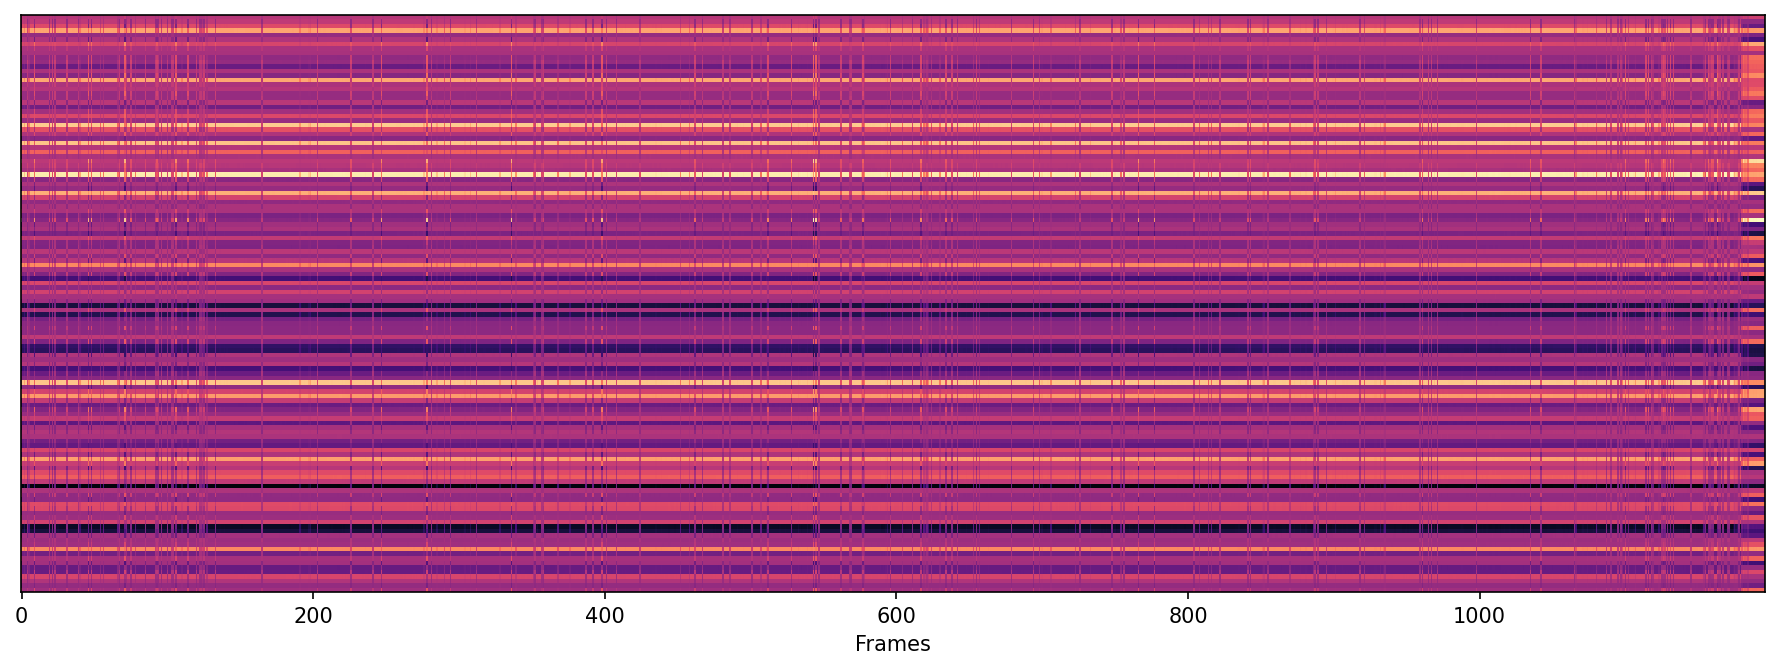
\includegraphics[width=\linewidth]{figures/images/355embeddiogramnormalized.png}
    \caption[Embeddiogram | Track 355 (SALAMI dataset).]{Embeddiogram. Track 355 (SALAMI dataset).}
    \label{fig:embeddiogram}
  \end{minipage}

  \begin{minipage}[b]{1.0\linewidth}
    \centering
    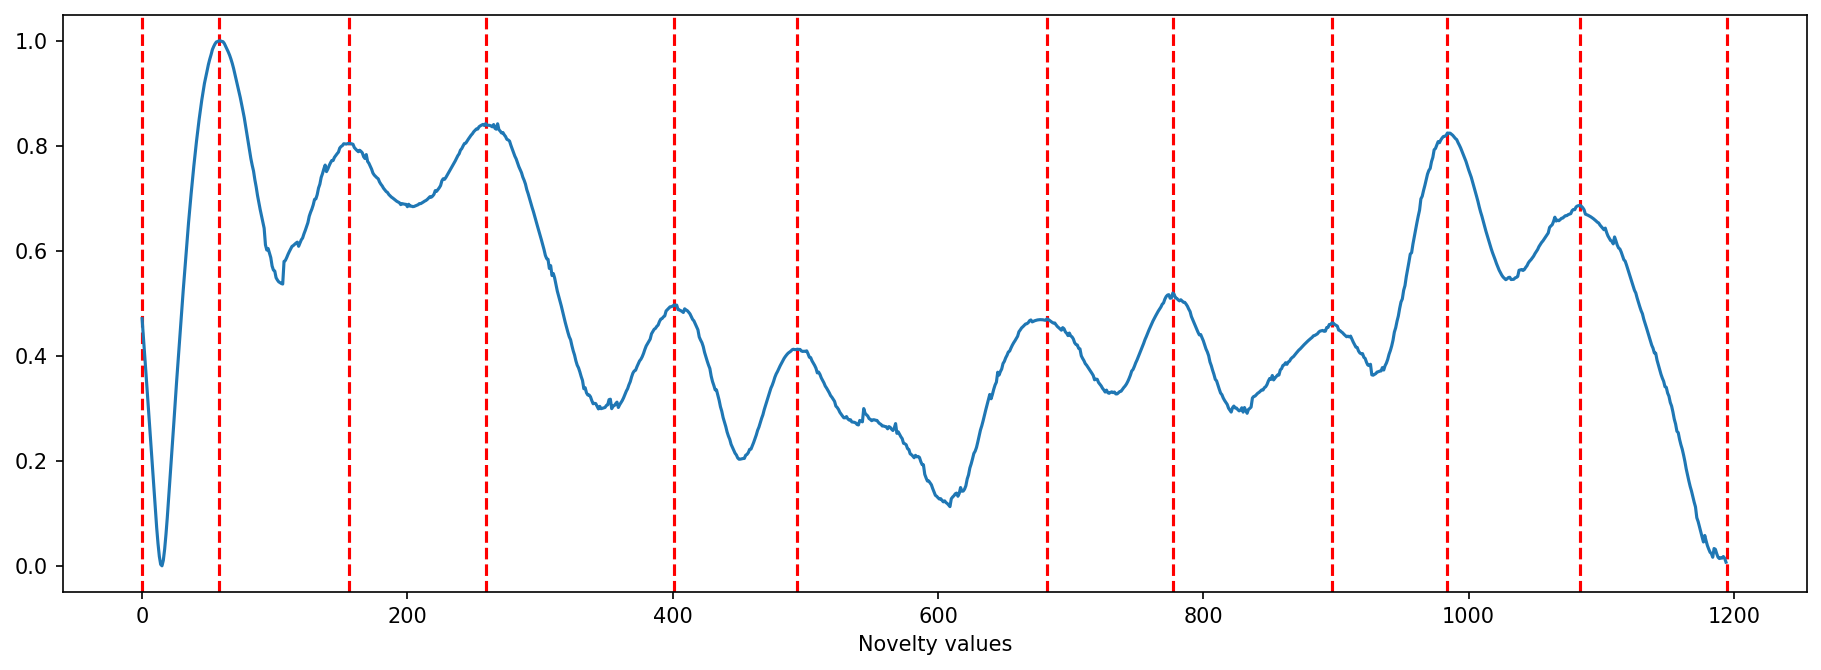
\includegraphics[width=\linewidth]{figures/images/355novelty.png}
    \caption[Novelty curve and peaks | Track 355 (SALAMI dataset).]{Novelty curve and peak detection. Track 355 (SALAMI dataset).}
    \label{fig:novelty}
  \end{minipage}
\end{figure}

\begin{figure}[ht]
    \centering
    \begin{minipage}{0.45\textwidth}
        \centering
        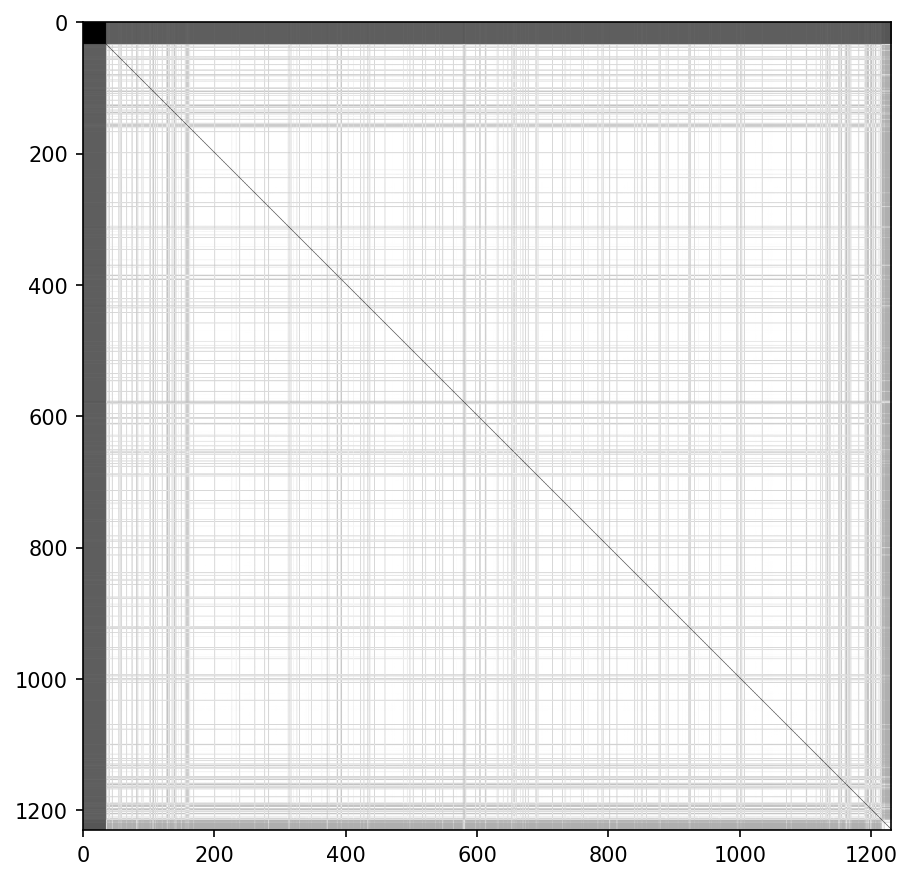
\includegraphics[width=0.9\textwidth]{figures/images/355recurrencematrix.png} % first figure itself
        \caption[Self-similarity matrix | Track 355 (SALAMI dataset)]{Self-similarity matrix computation of the embeddiogram. Track 355 (SALAMI dataset).}
        \label{fig:SSM}
    \end{minipage}\hfill
    \begin{minipage}{0.45\textwidth}
        \centering
        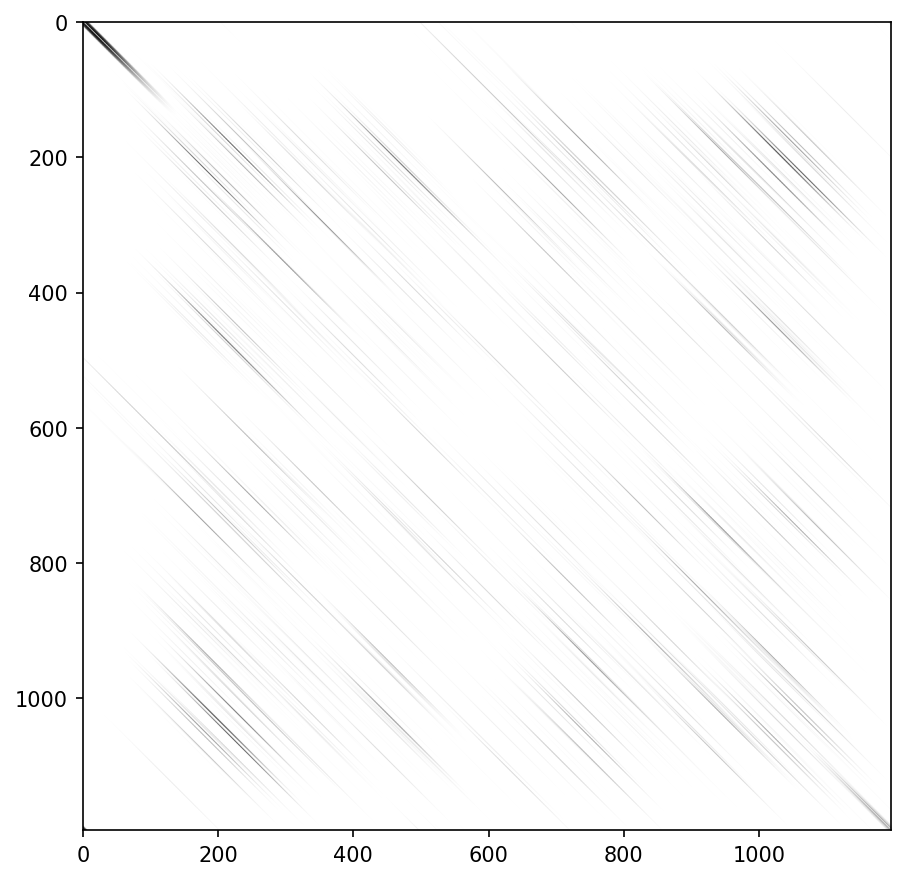
\includegraphics[width=0.9\textwidth]{figures/images/355lagmatrixgaussiansmoothing.png} % second figure itself
        \caption[Self-similarity lag matrix | Track 355 (SALAMI dataset)]{Self-similarity lag matrix. Track 355 (SALAMI dataset).}
        \label{fig:SSLM}
    \end{minipage}
    \vfill
    \begin{minipage}{0.45\textwidth}
        \centering
        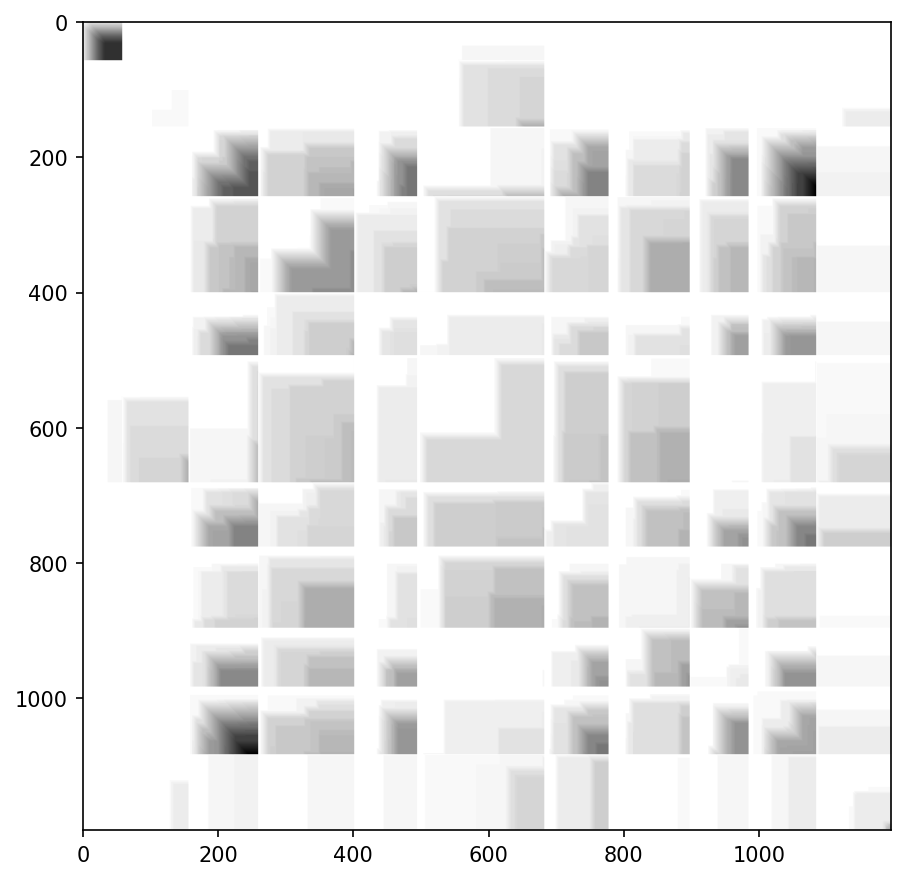
\includegraphics[width=0.9\textwidth]{figures/images/355cumulativematrix.png} % third figure itself
        \caption[Q-matrix | Track 355 (SALAMI dataset)]{Cumulative matrix computation of the embeddiogram. Track 355 (SALAMI dataset) .}
        \label{fig:Q}
    \end{minipage}\hfill
    \begin{minipage}{0.45\textwidth}
        \centering
        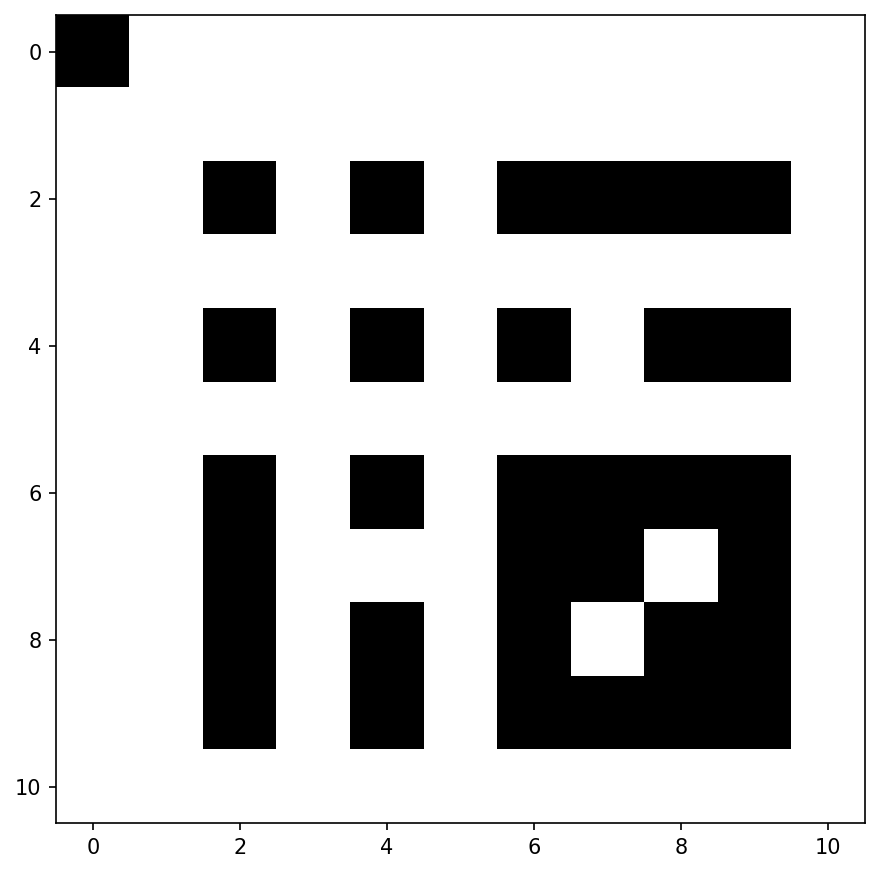
\includegraphics[width=0.9\textwidth]{figures/images/355transitivebinarysimilaritymatrix.png} % fourth figure itself
        \caption[Transitive Binary Similarity Matrix | Track 355 (SALAMI dataset)]{Transitive Binary Matrix computation of the embeddiogram. Track 355 (SALAMI dataset).}
        \label{fig:TBSM}
    \end{minipage}
\end{figure}

%%%%%%%%%%%%%%%%%%%%%%%%%

These deep audio features can be a foundation for current state-of-the-art methods, which are expected to receive as input standard traditional audio features. Consequently, they can be processed and manipulated like conventional features as described by \cite{unsuperMSA} and displayed in Figures \ref{fig:novelty}, \ref{fig:SSM}, \ref{fig:SSLM}, \ref{fig:Q}, and \ref{fig:TBSM}. Employing such embeddings in a traditional music segmentation algorithm can achieve state-of-the-art performance \cite{deepfeaturesegment}.

\newpage